\section{Wstępna analiza danych}
% Delete the text and write your Method(s) here:
%------------------------------------
\hspace{\parindent}

Po wstępnym oczyszczeniu naszych danych mamy następujący stosunek poszczególnych kategorii do wszystkich rekordów:\footnote{classification.ipynb}

\begin{figure}[H]
    \centering
    \includegraphics[width=0.5\textwidth]{Images/Podział kategorii.png}
    \label{fig:podzial-kategorii}
\end{figure}
Jak widzimy na diagramie, kategorie są prawie w identycznych proporcjach, co pozwoli na lepsze wytrenowanie modeli.

Sprawdzmy teraz zależność między poszczególnymi atrybutami a kategoriami:

\begin{figure}[H]
    \centering
    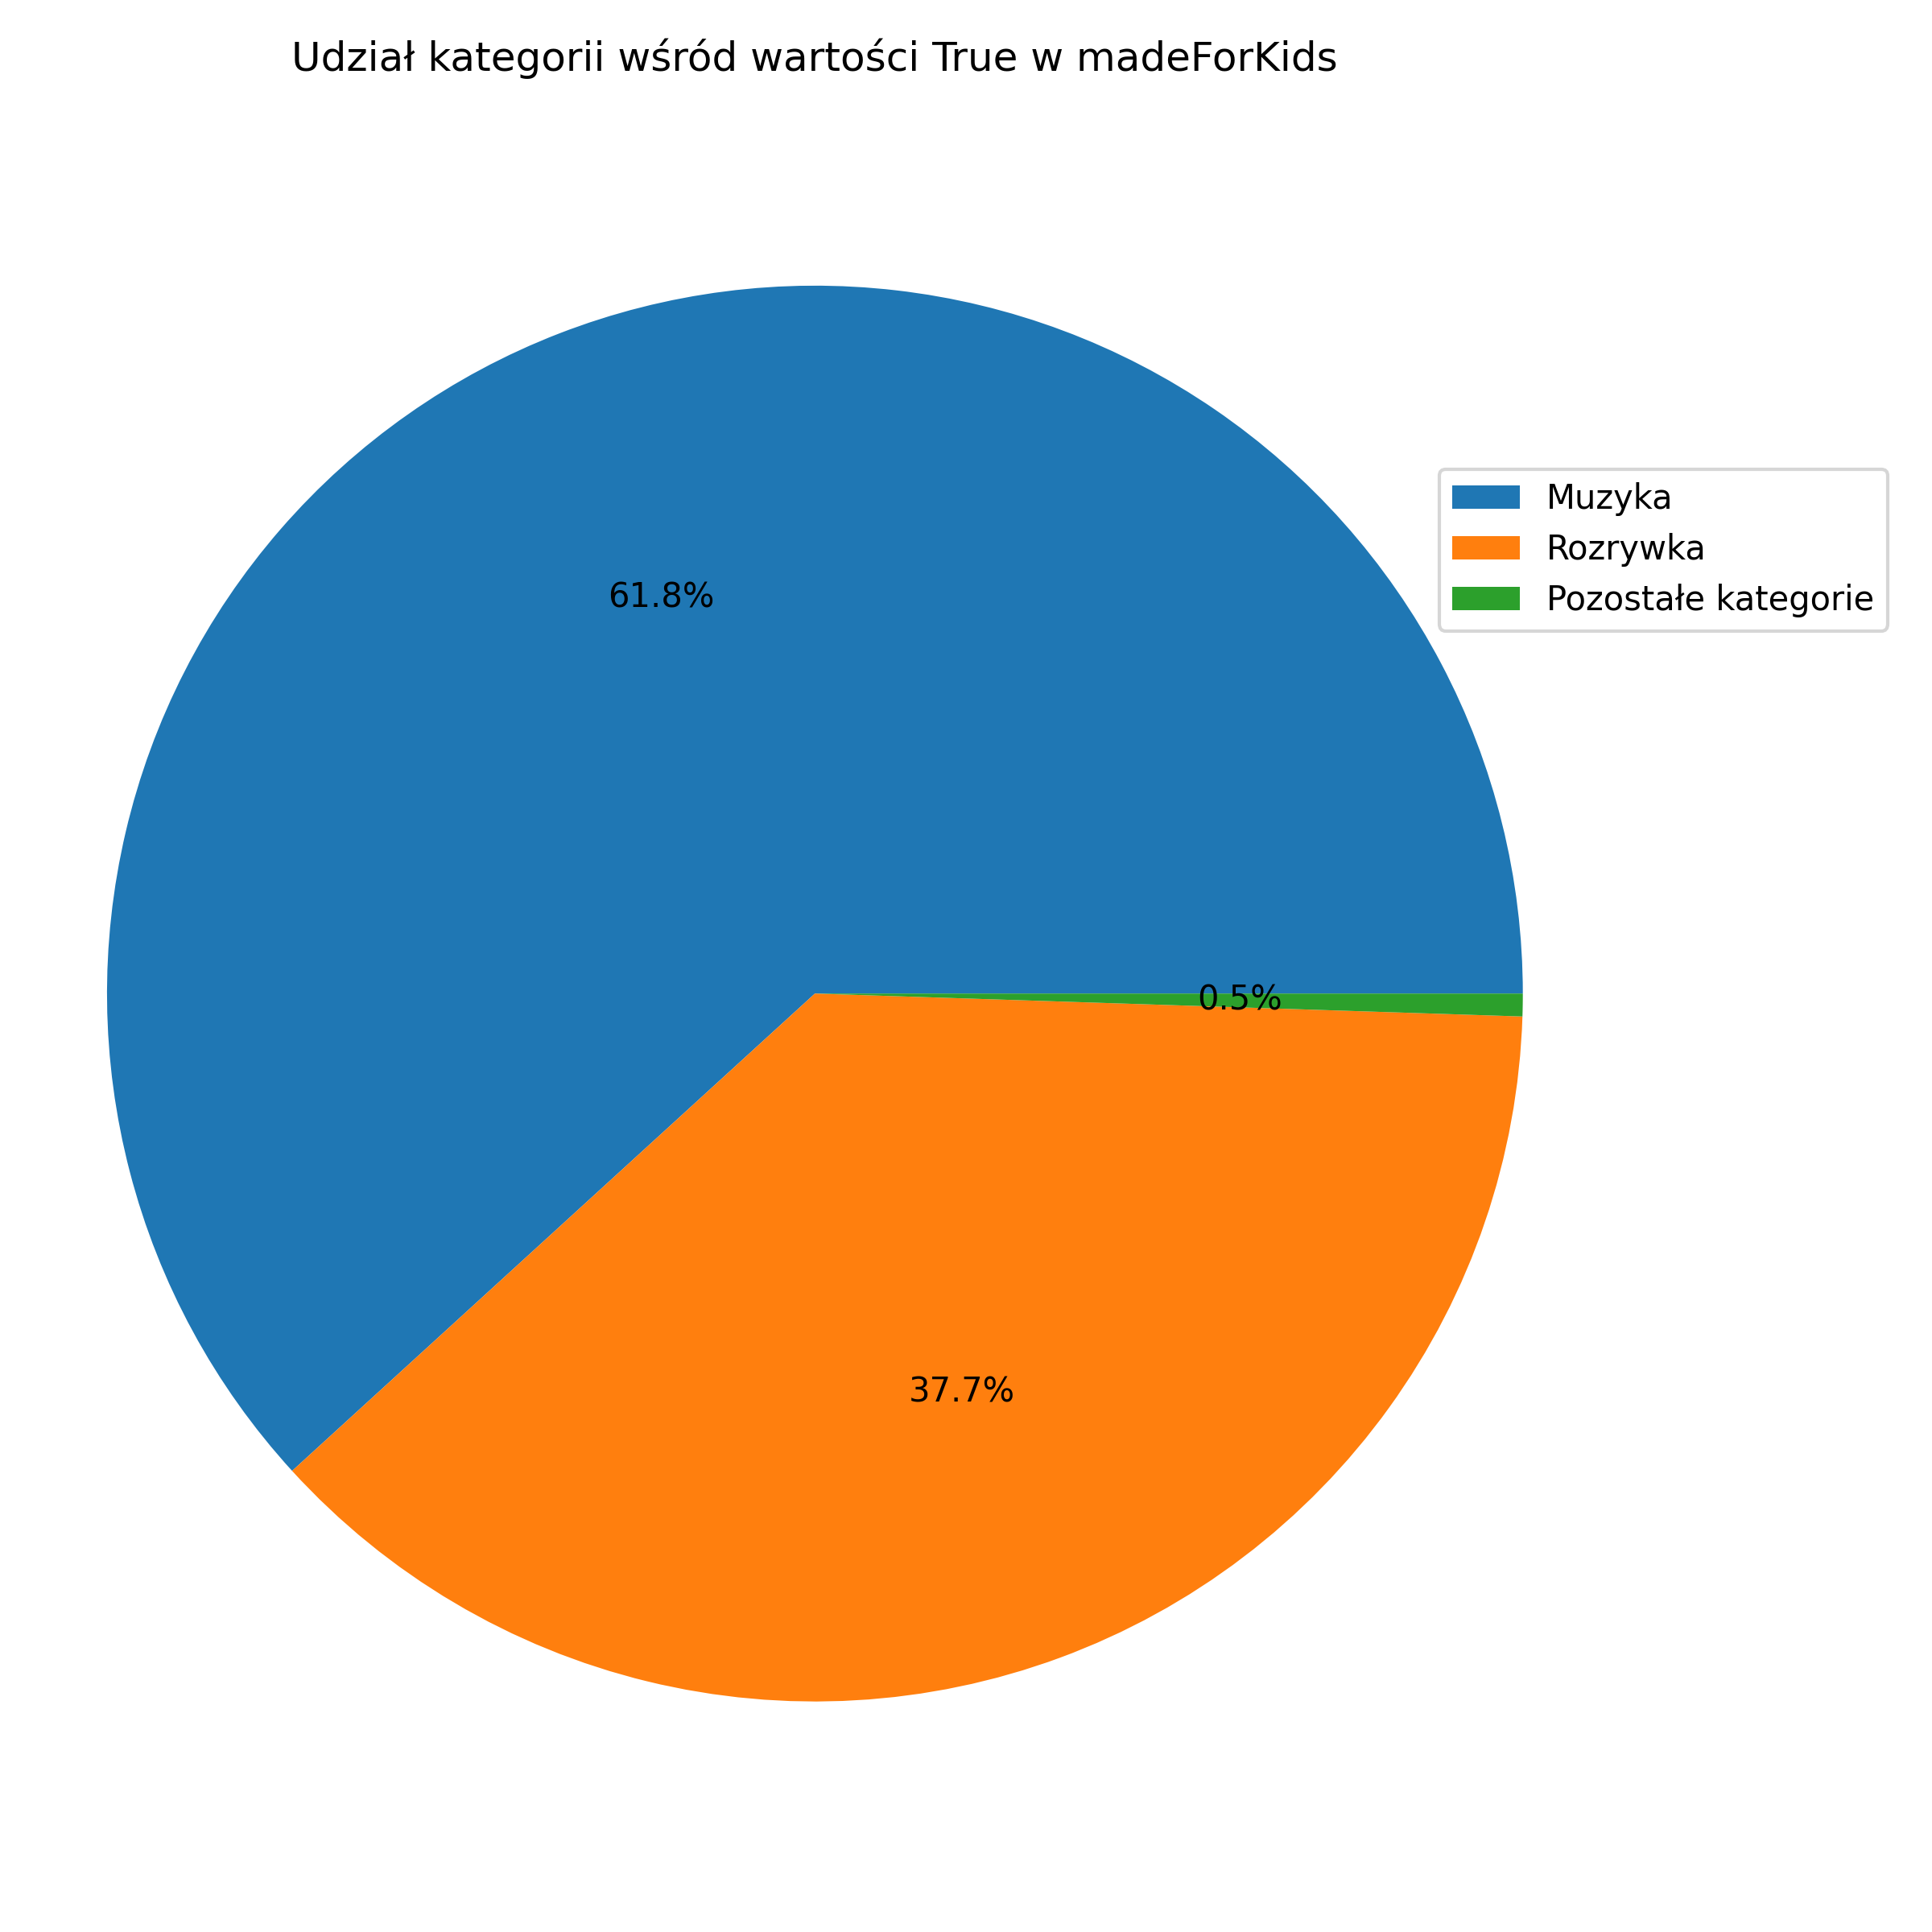
\includegraphics[width=0.5\textwidth]{Images/Diagram_true_do_reszty.png}
    \label{fig:madeforkids-true}
\end{figure}
Widzimy, że wartość true w atrybucie "Czy dla dzieci" pozwala nam w 99.5\% określić, że będą to dwie kategorie z pięciu, dokładniej mamy 61.8\% szans, że będzie to muzyka i 37.7\%, że będzie to rozrywka.

\begin{figure}[H]
    \centering
    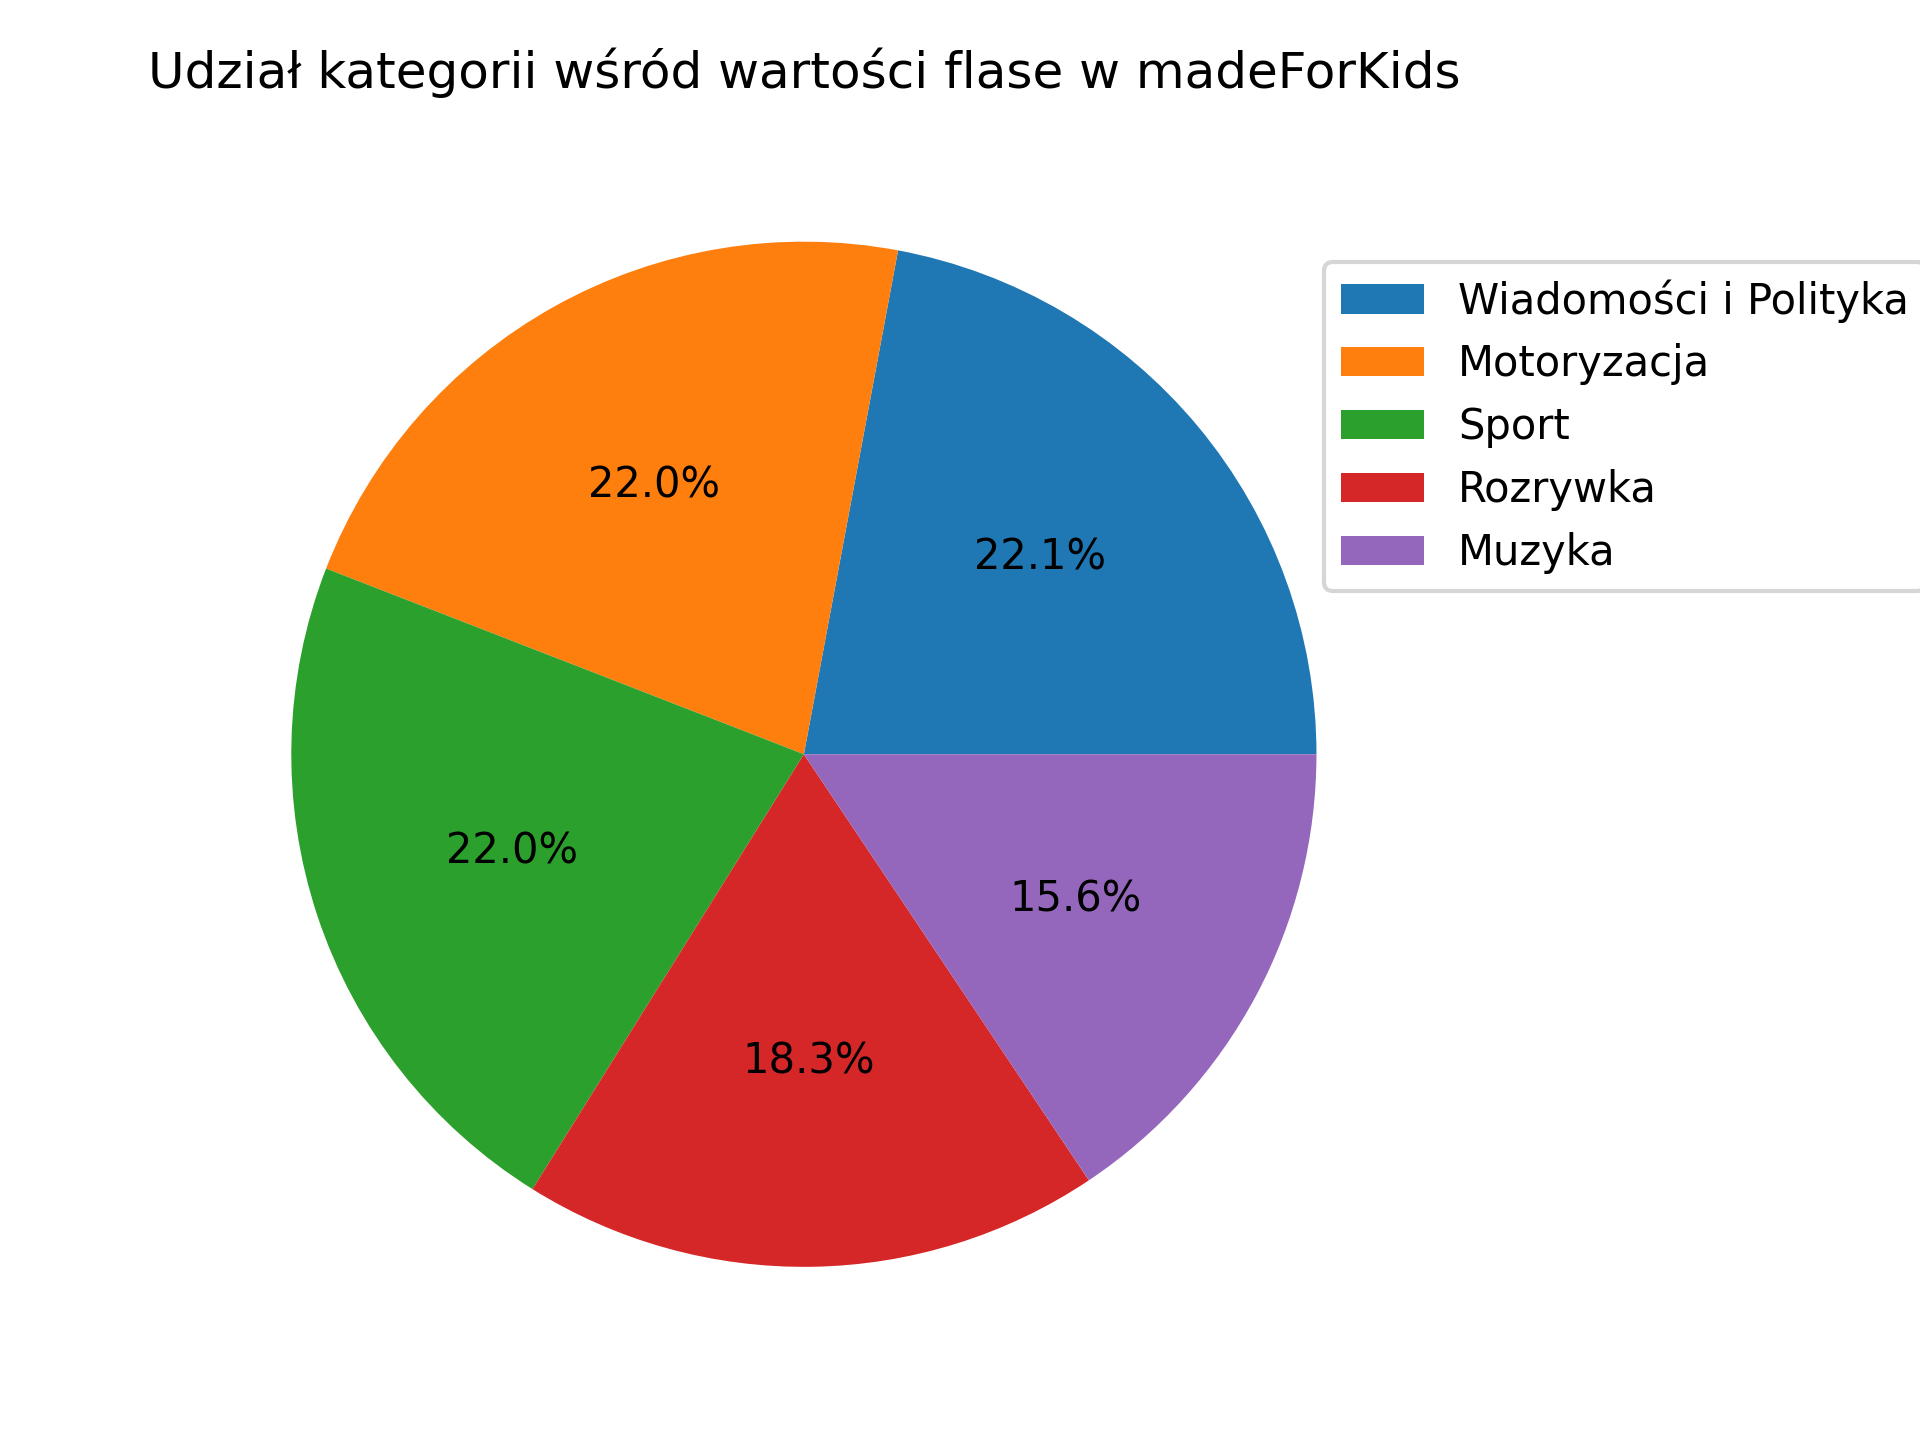
\includegraphics[width=0.5\textwidth]{Images/Diagram_false_do_reszty.png}
    \label{fig:madeforkids-false}
\end{figure}
Niestety dla wartości false widzimy, że nie ma tak znacznych różnic pomiędzy kategoriami.

\begin{figure}[H]
    \centering
    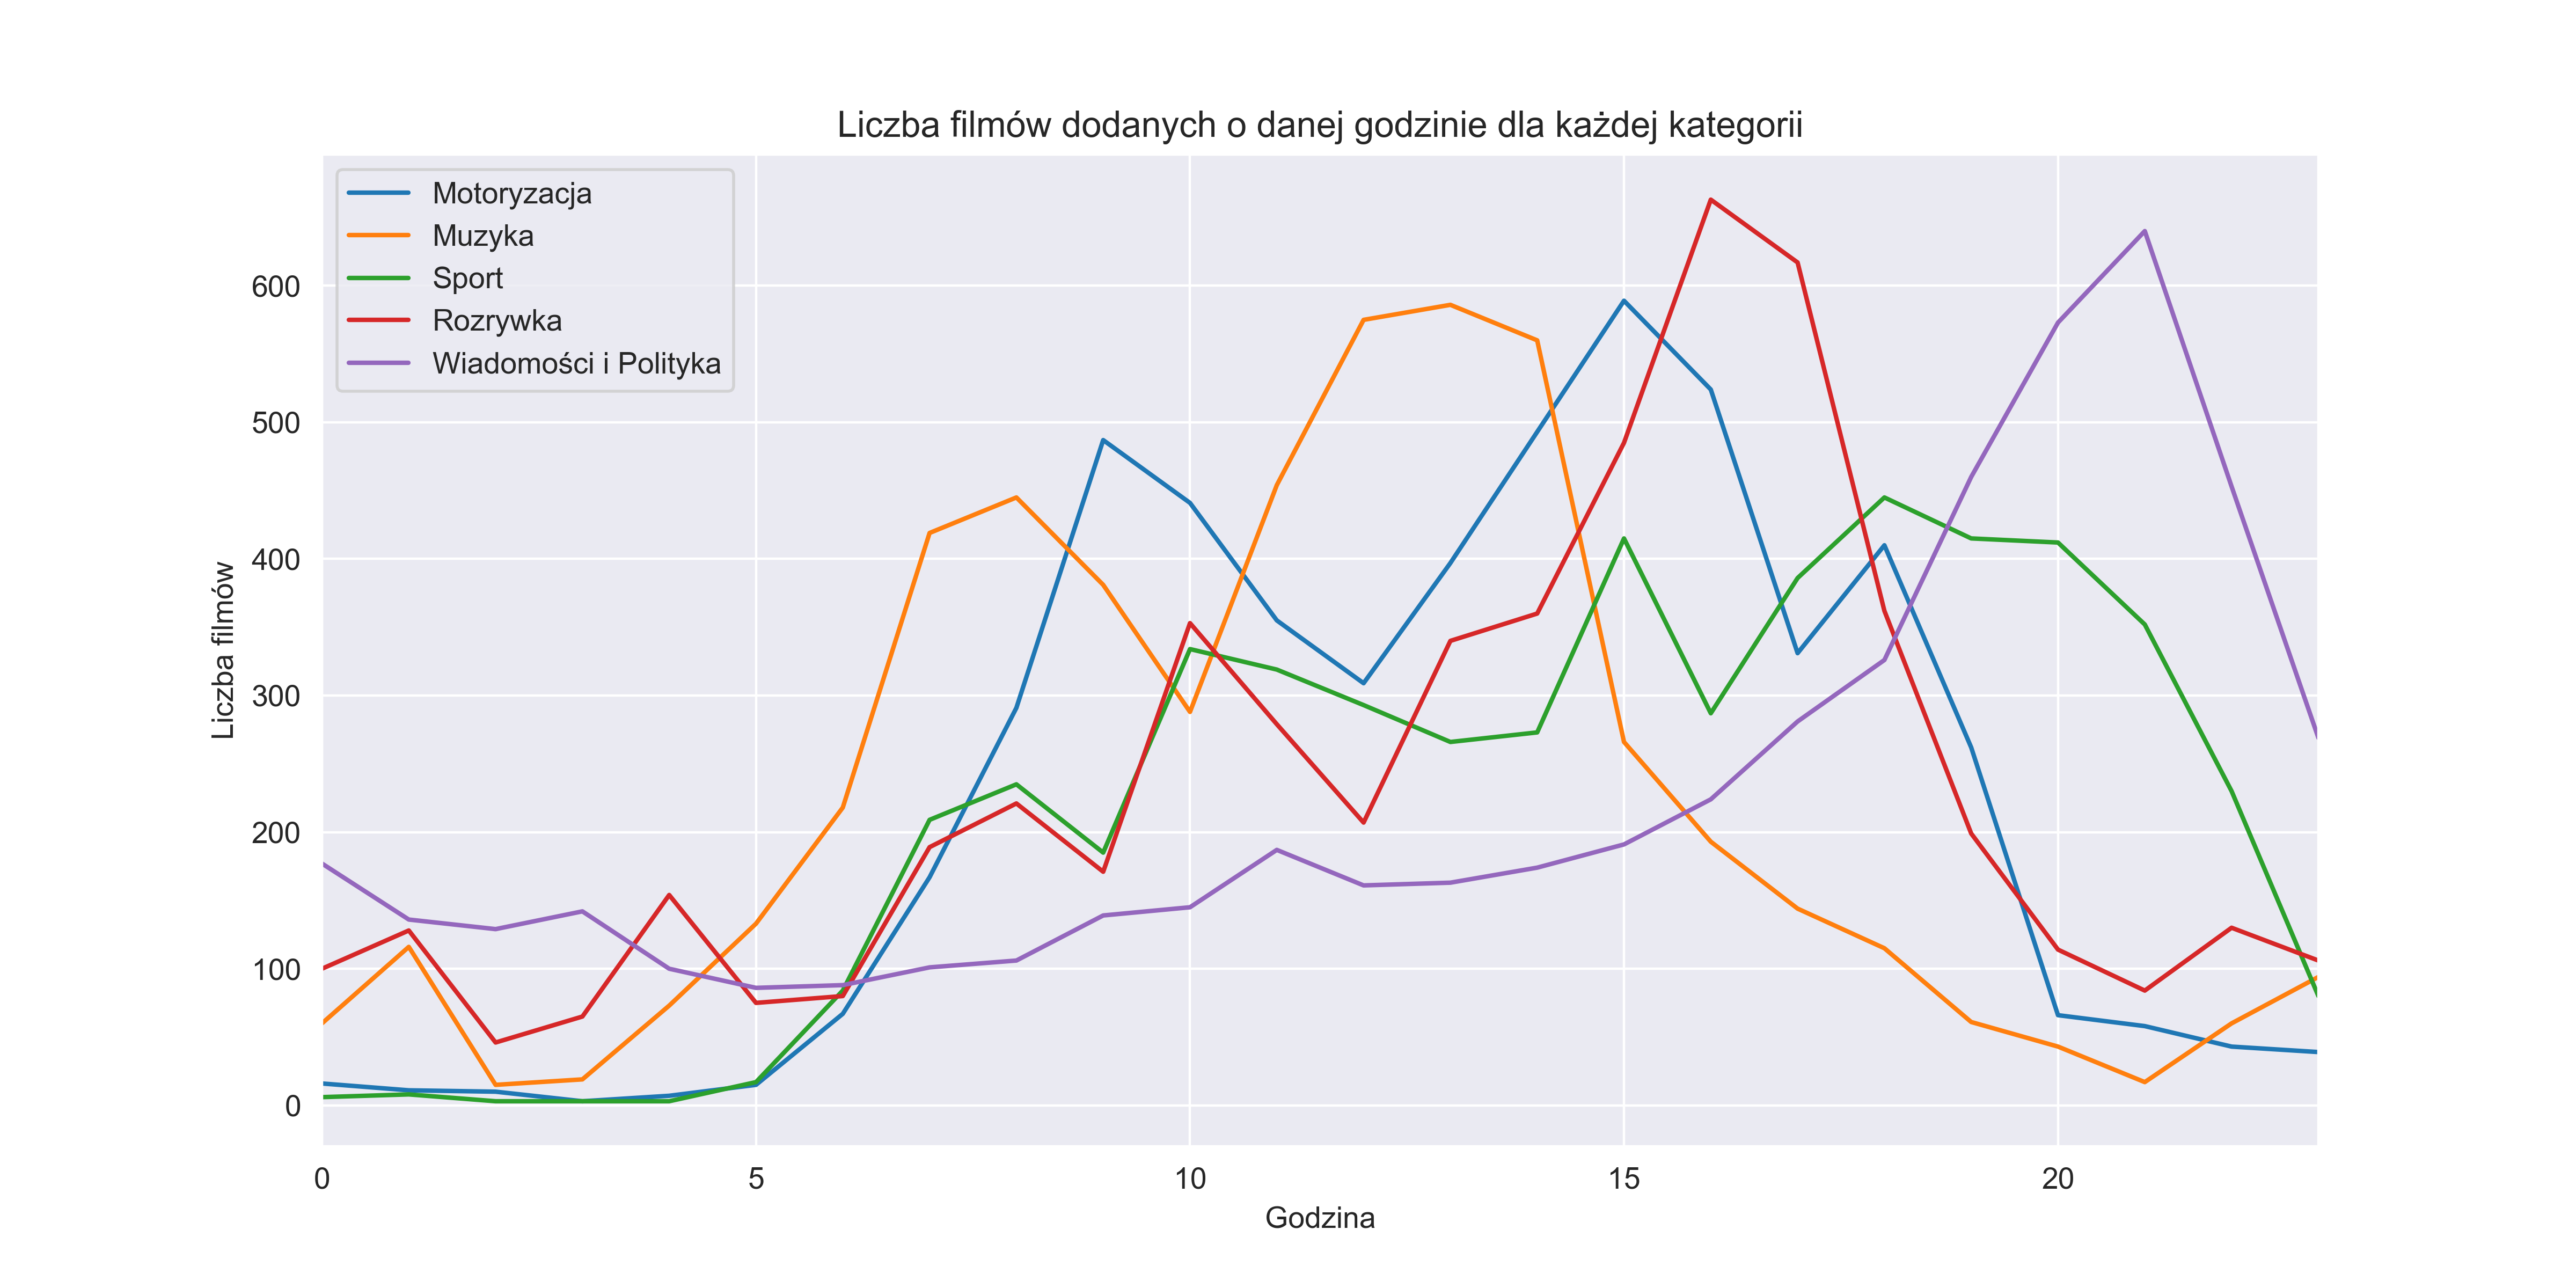
\includegraphics[width=0.5\textwidth]{Images/Zależność_dodania_do_filmu_a_kategorią.png}
    \label{fig:add_film_hour}
\end{figure}
Ten diagram bardzo dużo nam mówi o kategoriach, możemy się z niego dowiedzieć, że filmy z kategorii "Wiadomości i polityka" wrzucane są zazwyczaj w okolicach godziny 21. Natomiast kategoria sport nie ma jednej godziny, w której najczęściej wrzucane są filmy. Pozostałe trzy kategorie mają bardzo podobne wykresy z delikatnym przesunięciem.

\begin{figure}[H]
    \centering
    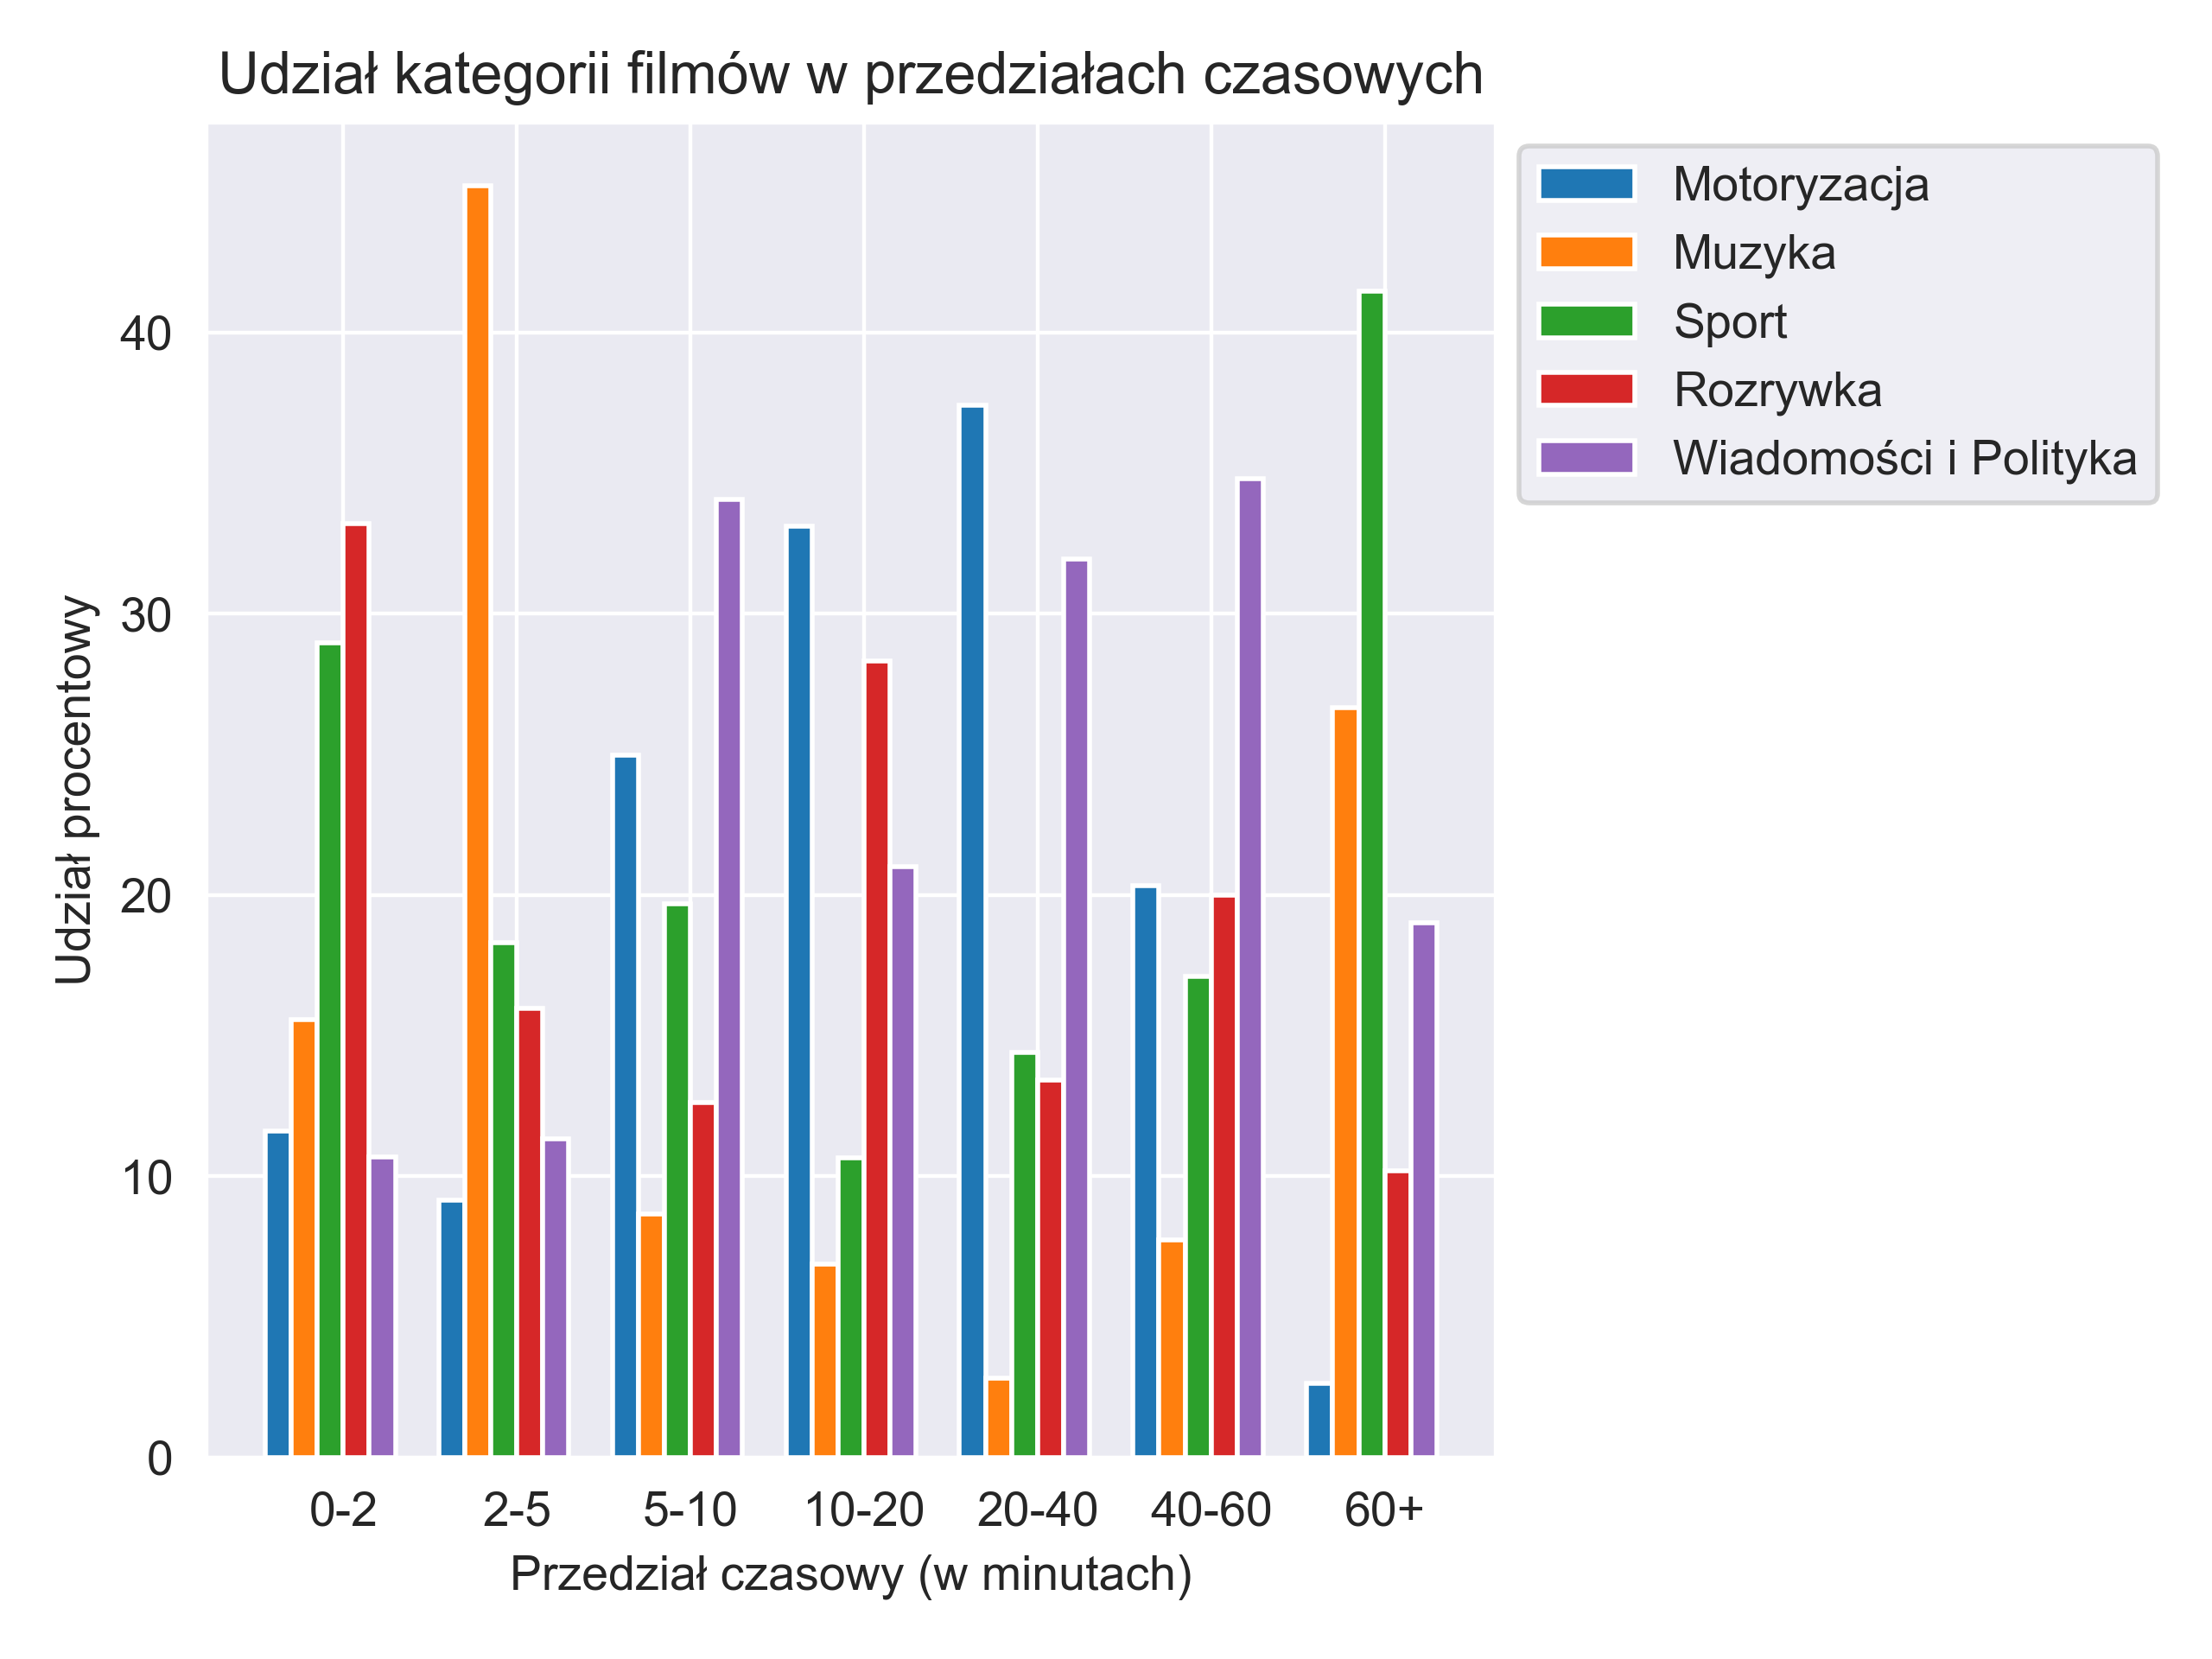
\includegraphics[width=0.5\textwidth]{Images/Udział kategorii filmów w przedziałach czasowych.png}
    \label{fig:durations}
\end{figure}
Wykres przedstawia udział poszczególnych kategorii w konkretnych przedziałach czasowych, co pozwala nam na przykład określić, że jeśli film trwa pomiędzy 2-5 minut, to na 45\% będzie to film z kategorii muzyka.


\begin{figure}[H]
    \centering
    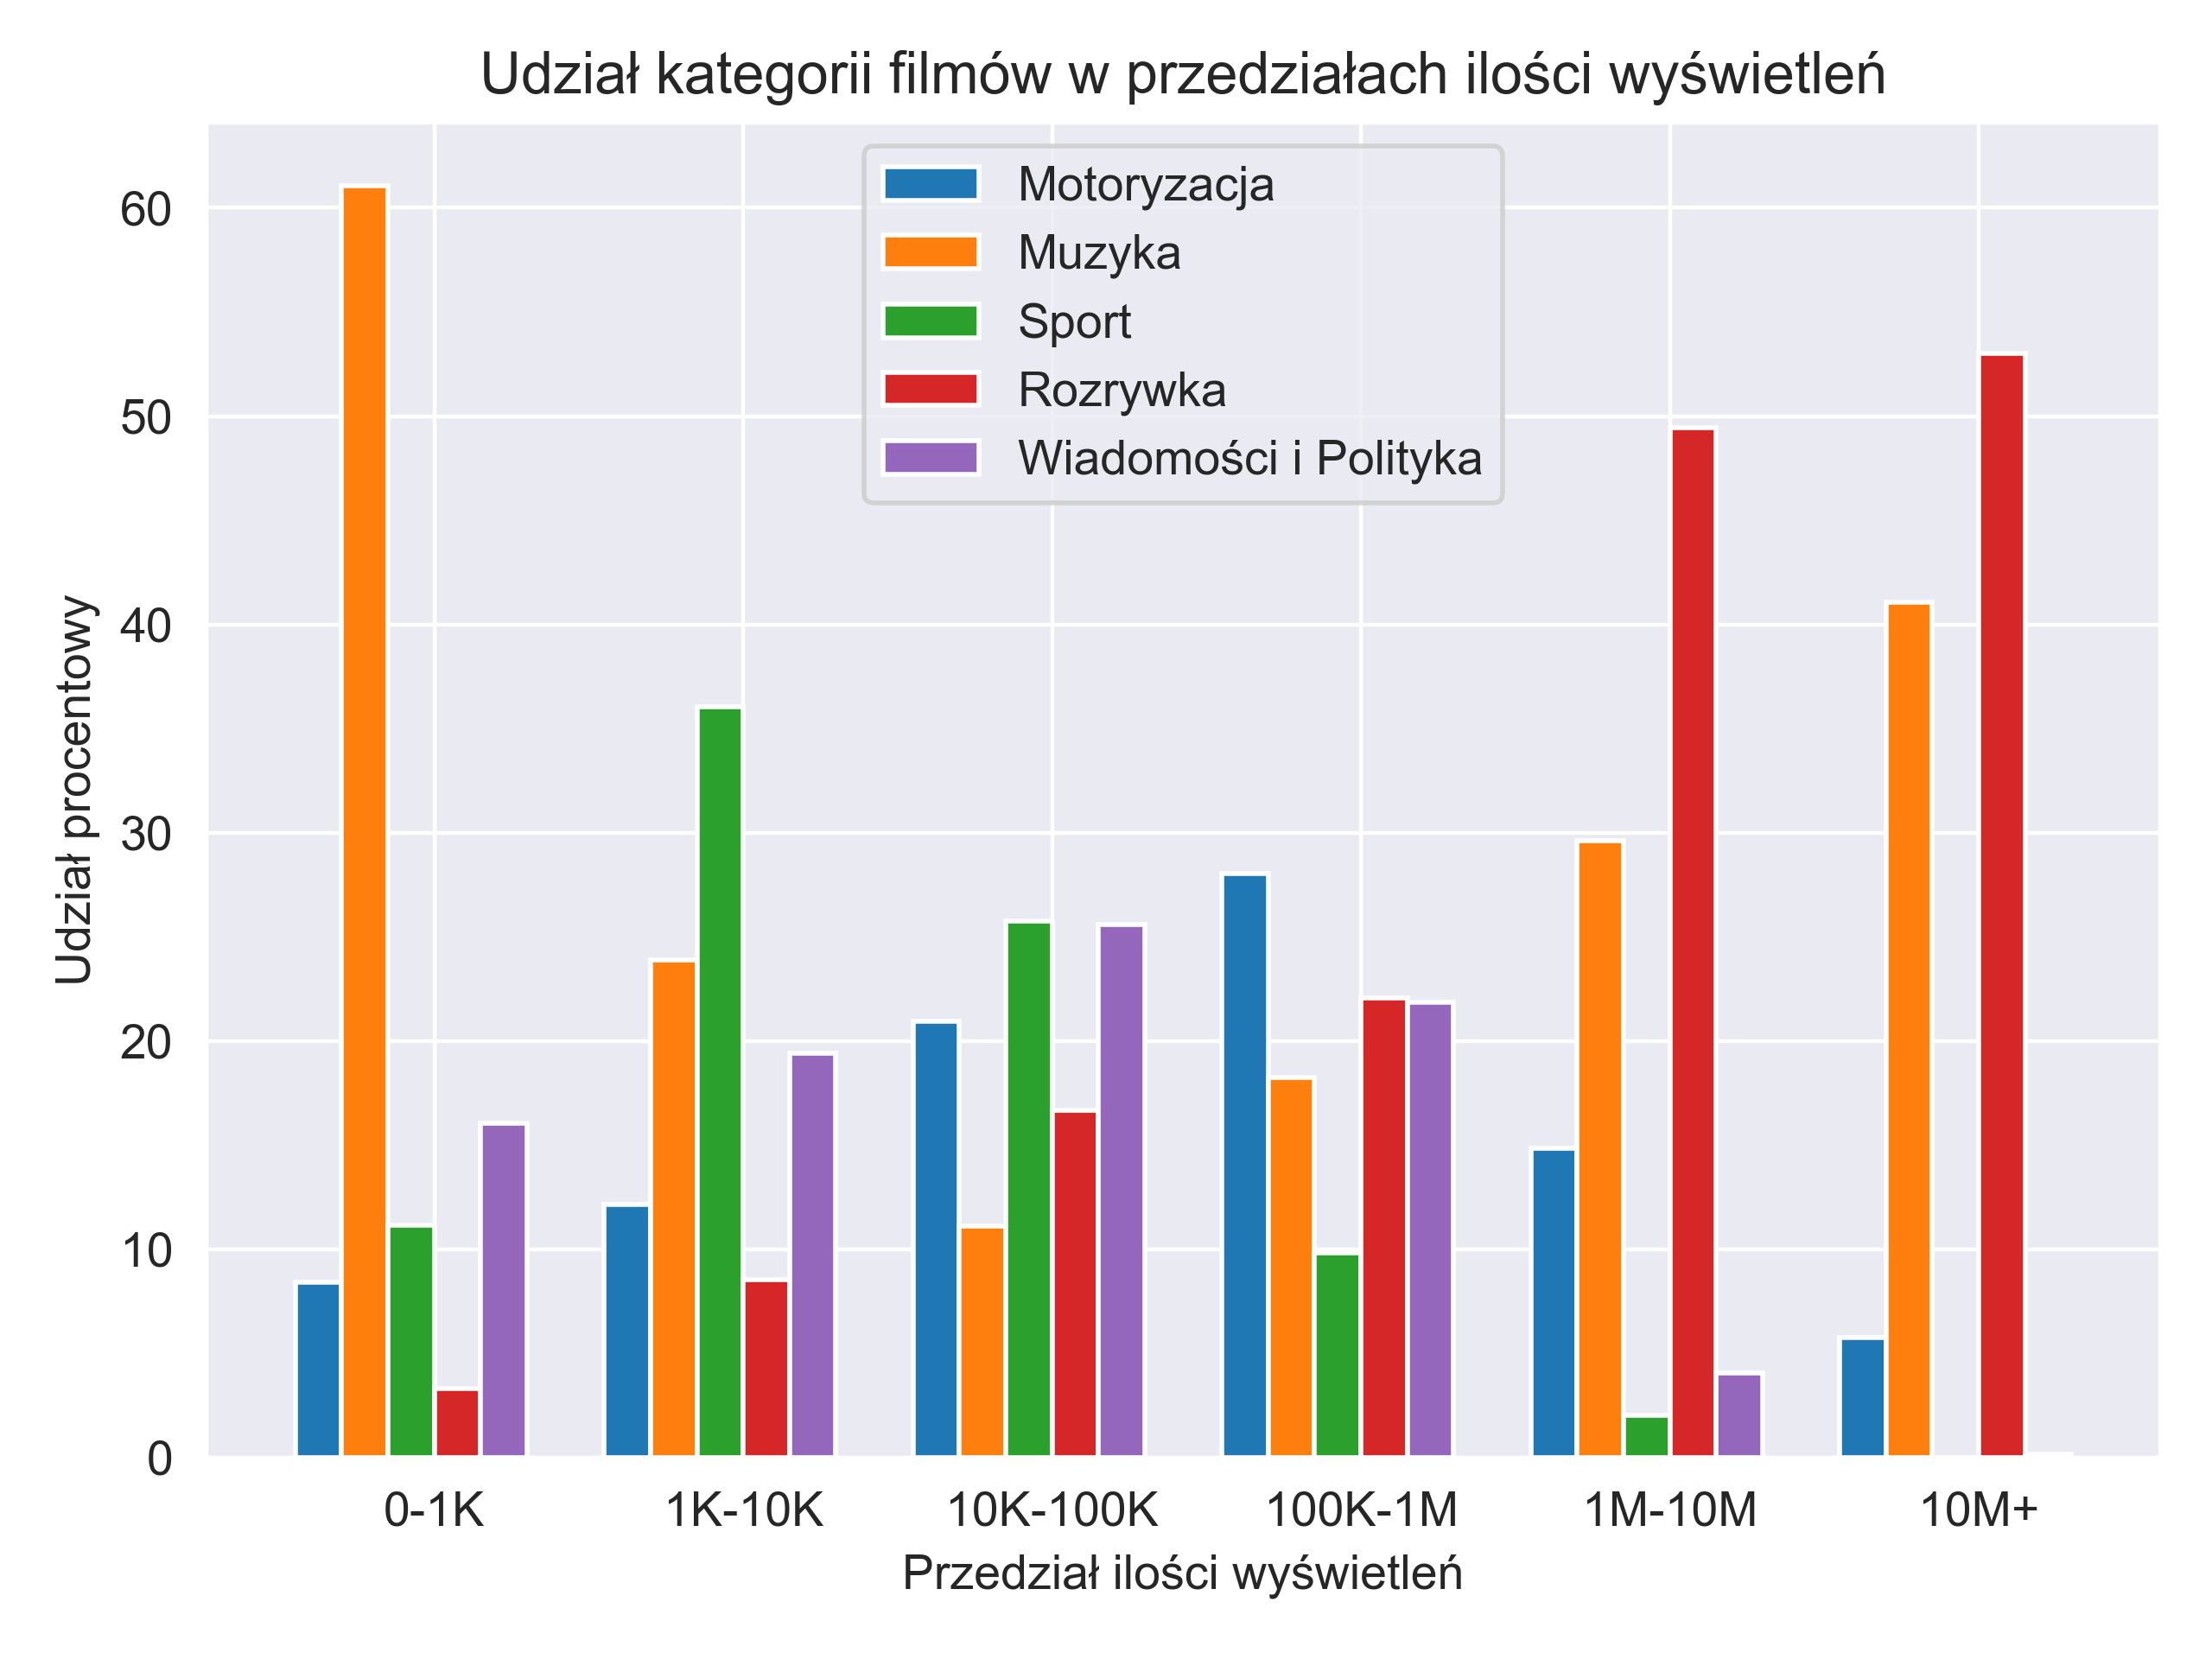
\includegraphics[width=0.5\textwidth]{Images/Zależność wyświetleń od kategorią.png}
    \label{fig:views_count}
\end{figure}
Następny diagram przedstawia zależność między kategoriami, a ilością wyświetleń w przedziałach. Widzimy, że środkowe przedziały dużo nam nie mówią, bo wszystkie kategorie mają podobną ilość wyświetleń, natomiast skrajne, takie jak 0-1k pozwalają nam dostrzec, że za 60\% wyświetleń w tym przedziale odpowiada kategoria muzyka lub, że w przedziale 10M+ nie występują kategorie Wiadomości i polityka oraz sport, a motoryzacja odpowiada tylko za 5\%.

\begin{figure}[H]
    \centering
    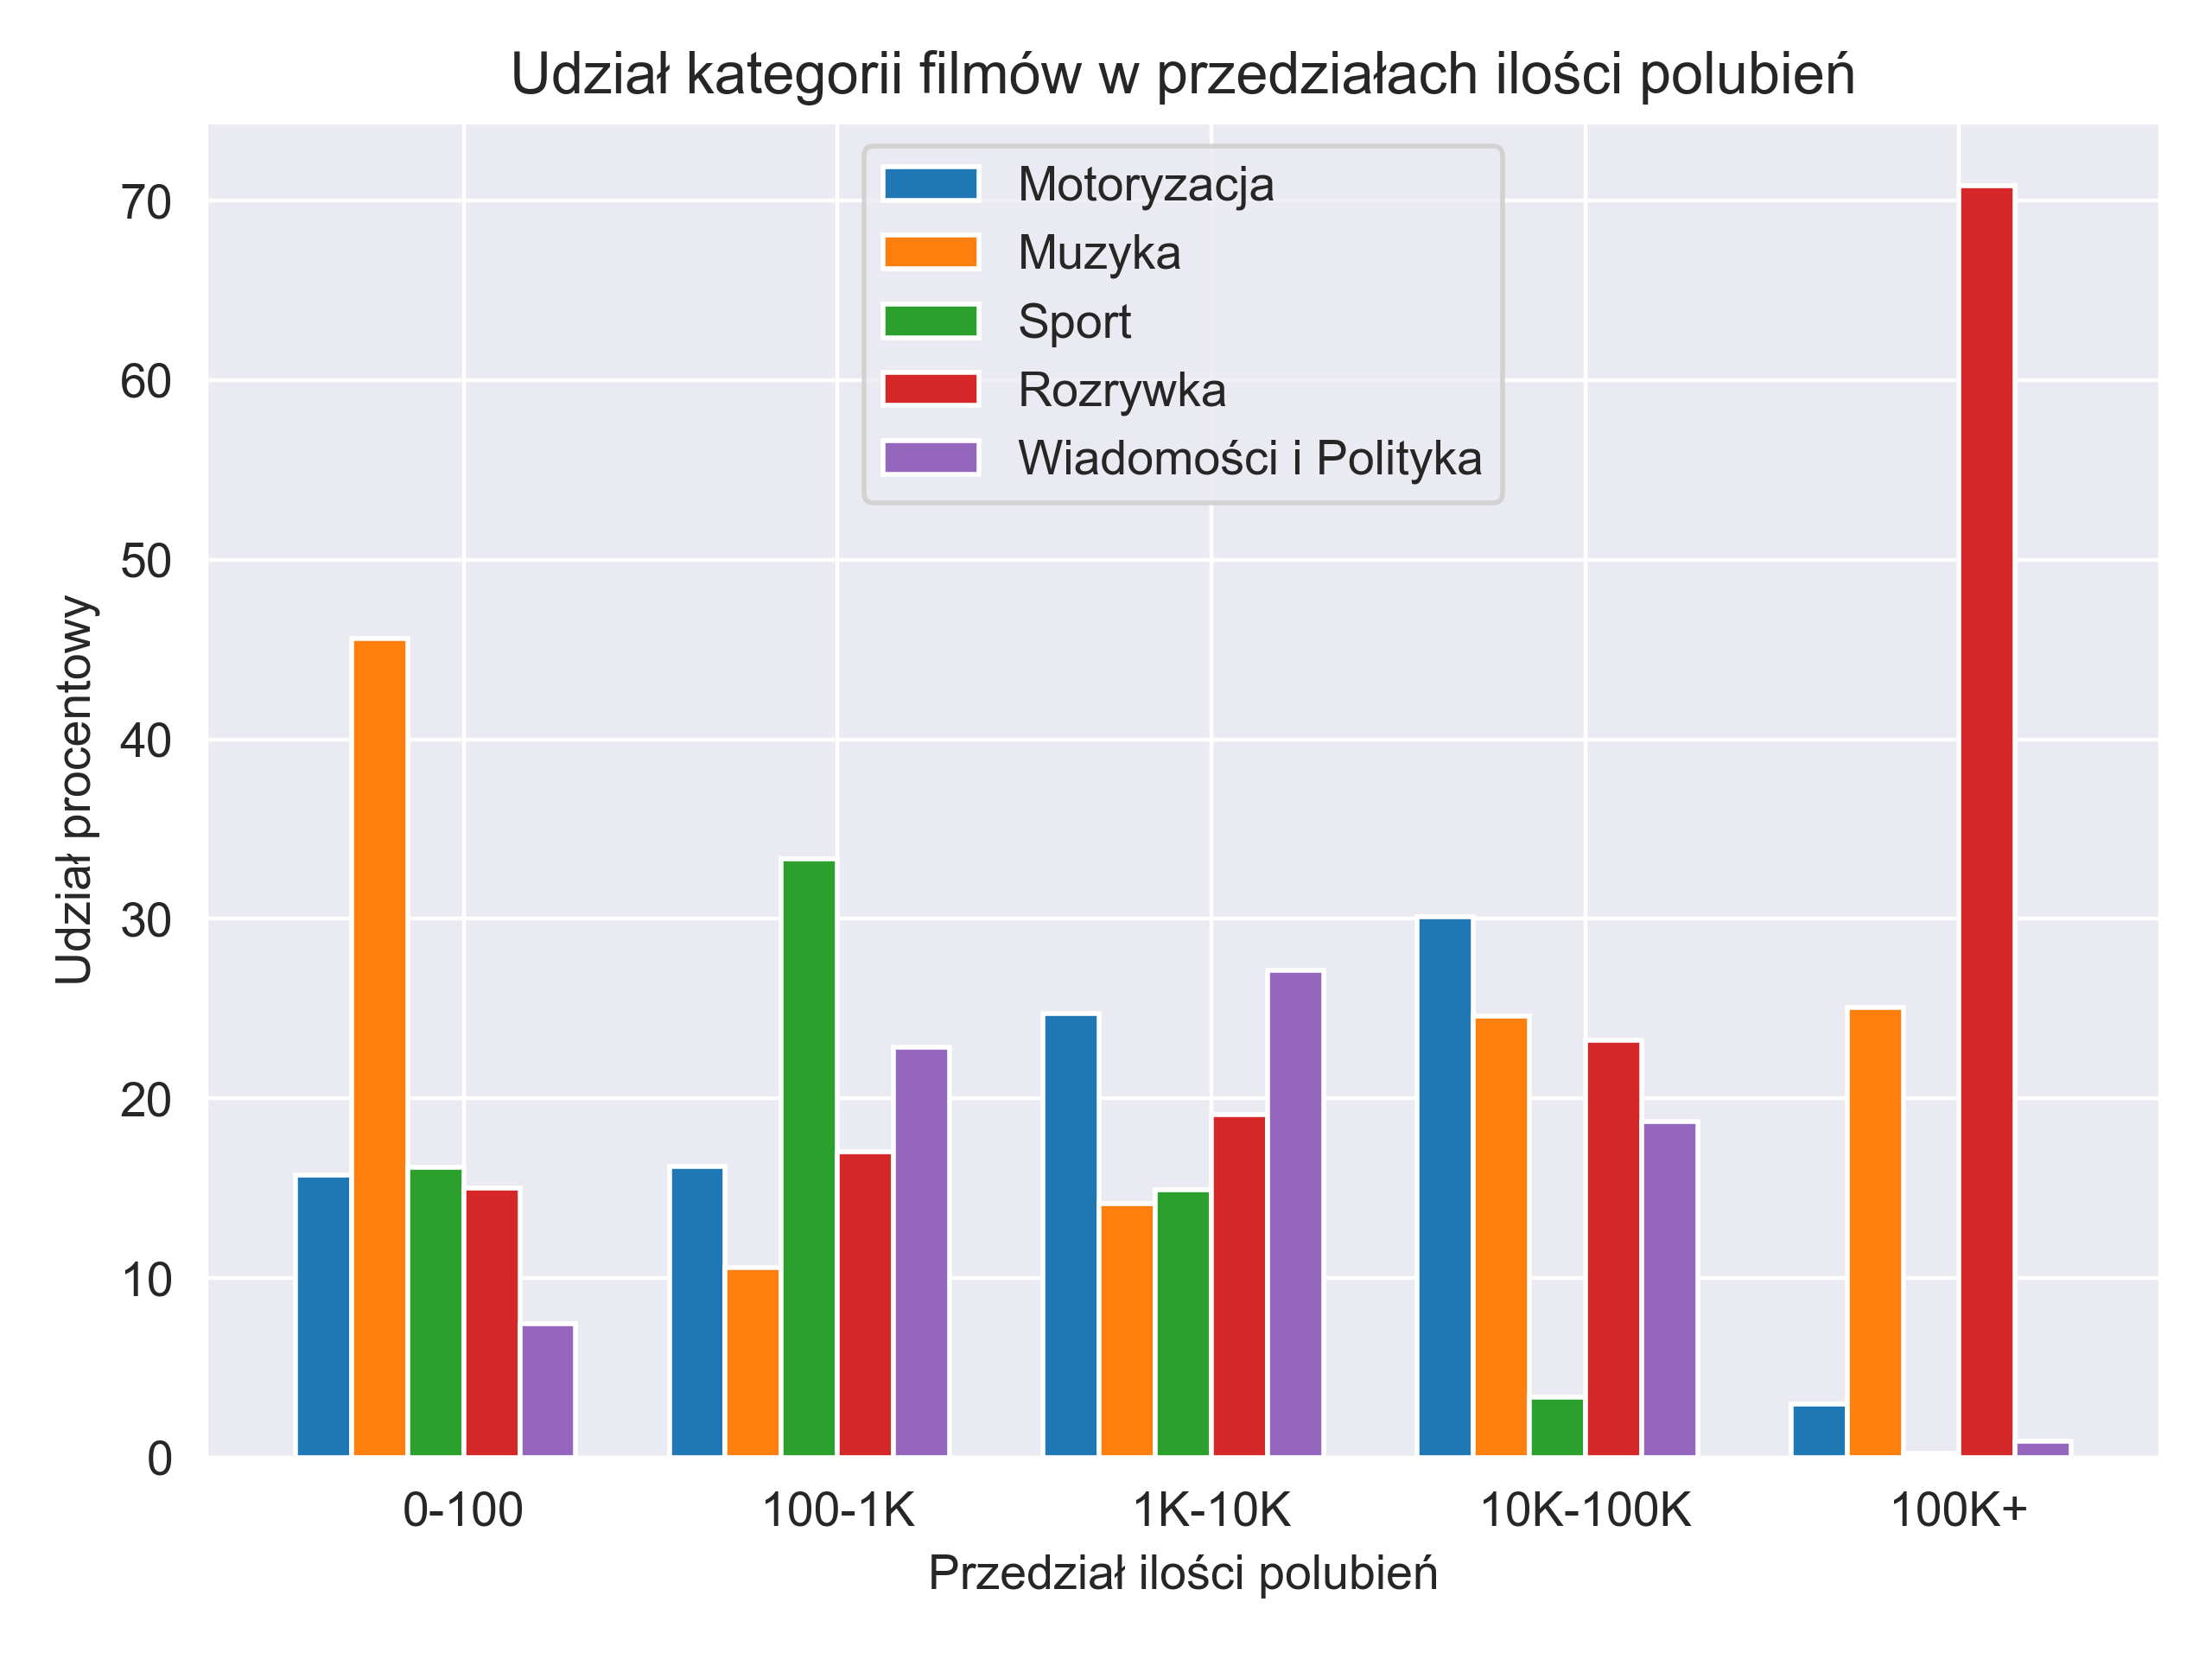
\includegraphics[width=0.5\textwidth]{Images/Zależność polubień od kategorią.png}
    \label{fig:likes_count}
\end{figure}
Ten diagram jest bardzo podobny do poprzedniego, ponieważ tutaj również nie widzimy dużych różnic pomiędzy kategoriami w środkowych przedziałach. Natomiast skrajne kategorie również dostarczają nam bardzo zróżnicowanych wyników, takich jak 70\% udziału kategorii rozrywka dla ilości polubień powyżej 100000.

\begin{figure}[H]
    \centering
    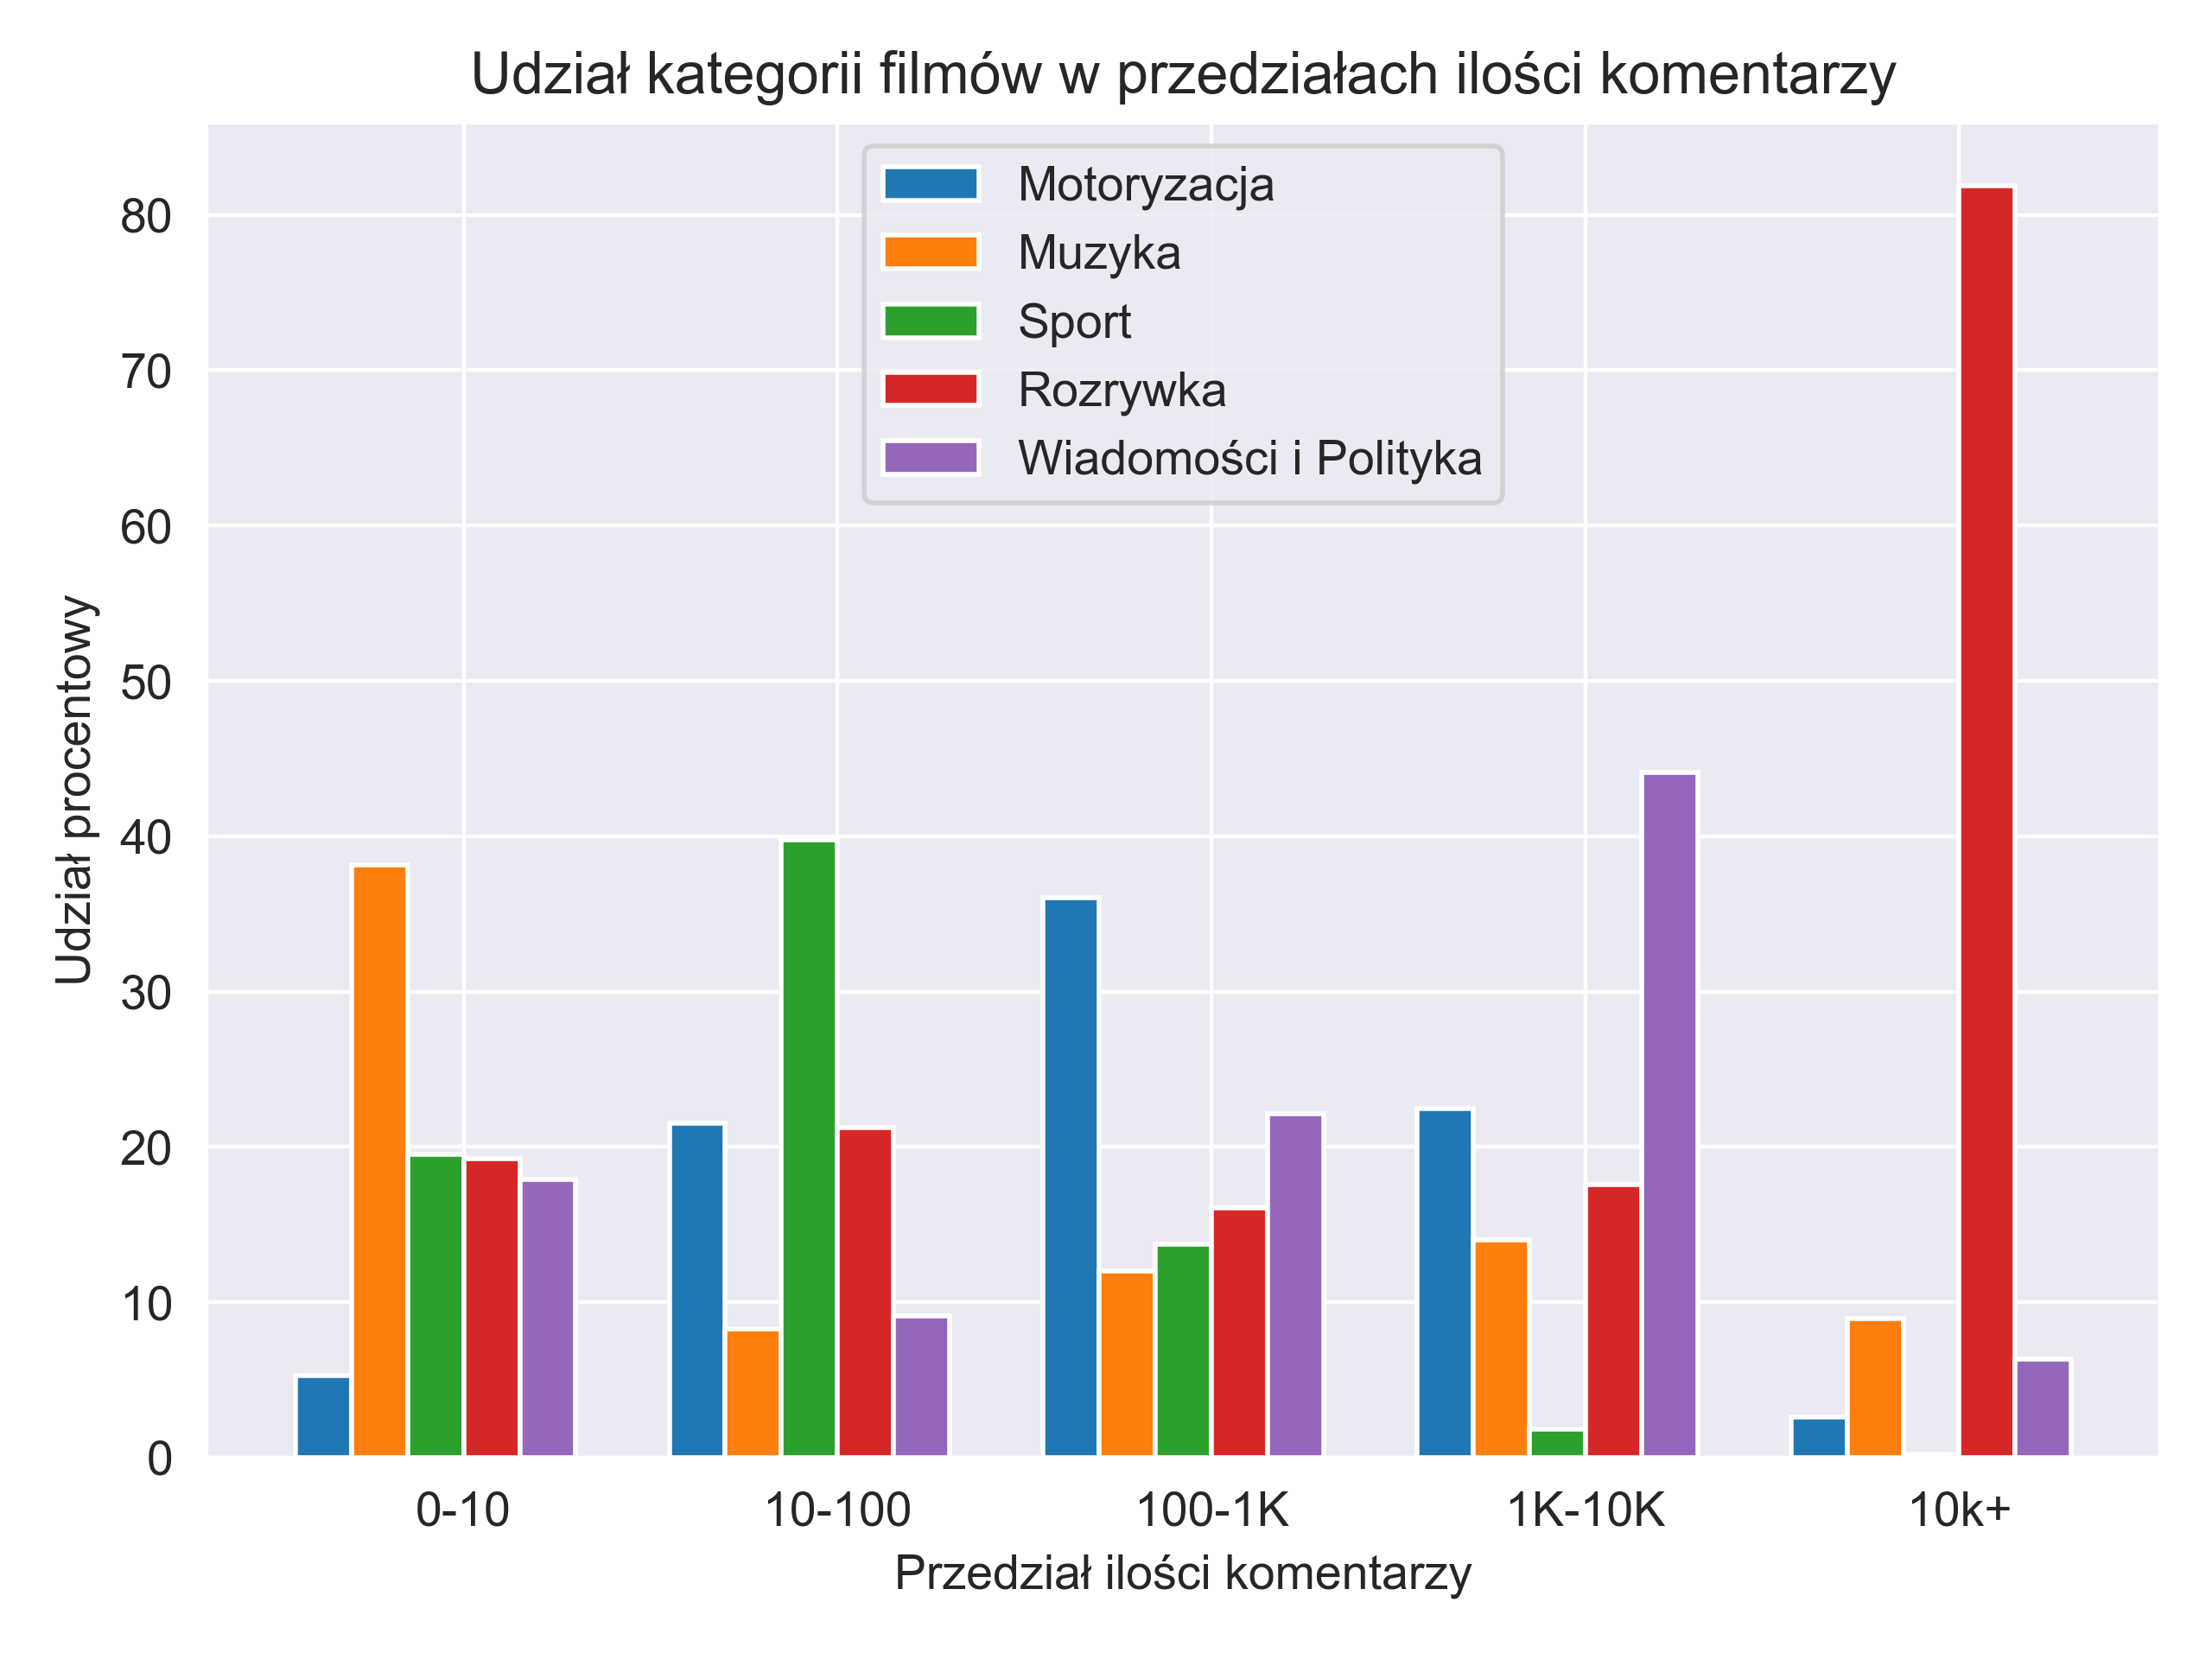
\includegraphics[width=0.5\textwidth]{Images/Zależność komentarzy od kategorią.png}
    \label{fig:coments_count}
\end{figure}
Przedostatni diagram przedstawiający zależność między atrybutami a kategoriami jest bardzo ciekawy, ponieważ tutaj w każdym przedziale inna kategoria dominuje o ponad 15\%. Jednak tak jak w dwóch ostatnich diagramach widać największą różnicę między kategoriami w górnym skrajnym przedziale, tak w tym przypadku jest to przedział ponad 10000, w którym kategoria rozrywka ma aż 80\% udziału.

\begin{figure}[H]
    \centering
    \includegraphics[width=0.5\textwidth]{Images/kategorię a dnia od 2012.png}
    \label{fig:add_days}
\end{figure}
Ostatni diagram przedstawia nam zależność między opublikowaniem filmu a kategorią. Możemy tutaj dostrzec, że zgromadzony przez nas zbiór nie jest idealny. Kategorie powinny się pokrywać, ponieważ codziennie są publikowane filmy z tych kategorii. Dlatego do uczenia naszego modelu nie bedziemy stosować tego atrybutu, tak aby nasz model był możliwy do wykorzystania dla najnowszych filmów i jak najlepiej działał na innych zbiorach.


